% !TEX root = ../sommaire.tex

\chapter{Introduction générale}

\section{Contexte et motivation}

\subsection{Organoïdes : révolution en biologie cellulaire et médecine régénérative}

Les organoïdes, ces structures tridimensionnelles cultivées \textit{in vitro} qui miment la complexité architecturale et fonctionnelle des organes humains, représentent une avancée majeure en biologie cellulaire et en médecine régénérative~\cite{Zhao2022}. Contrairement aux cultures cellulaires bidimensionnelles traditionnelles où les cellules sont forcées de croître sur des surfaces planes artificielles, les organoïdes reproduisent l'organisation spatiale tridimensionnelle, les interactions cellulaires complexes, les gradients biochimiques et l'architecture tissulaire caractéristiques des tissus \textit{in vivo}.

Depuis leur première description pour l'intestin en 2009 par l'équipe de Hans Clevers~\cite{Sato2009}, les organoïdes ont été développés pour de nombreux organes : cerveau, rein, foie, poumon, pancréas, rétine, et bien d'autres. Ces mini-organes auto-organisés, typiquement de quelques centaines de micromètres à quelques millimètres de diamètre, peuvent être générés à partir de cellules souches embryonnaires (ESC), de cellules souches pluripotentes induites (iPSC), ou de cellules souches adultes résidentes dans les tissus.

La capacité des organoïdes à récapituler les processus développementaux, à maintenir l'hétérogénéité cellulaire des tissus natifs, et à répondre aux stimuli de manière physiologiquement pertinente en fait des modèles \textit{in vitro} sans précédent. Ils comblent le fossé entre les cultures cellulaires 2D simplistes et les modèles animaux complexes et coûteux, offrant un compromis optimal entre contrôle expérimental, pertinence biologique et accessibilité.

\subsection{Applications thérapeutiques et criblage de médicaments}

Les applications des organoïdes s'étendent de la recherche fondamentale au développement thérapeutique et à la médecine personnalisée.

\subsubsection{Modélisation de maladies}

En oncologie, les organoïdes tumoraux dérivés directement de biopsies de patients (patient-derived organoids, PDOs)~\cite{Drost2019} permettent de recréer \textit{in vitro} l'hétérogénéité tumorale et le microenvironnement tumoral. Ces modèles fidèles peuvent être utilisés pour tester \textit{ex vivo} l'efficacité de traitements personnalisés avant leur administration au patient, guidant ainsi les décisions thérapeutiques. Des biobanques d'organoïdes tumoraux sont actuellement constituées pour représenter la diversité génétique et phénotypique des cancers.

Dans le domaine des maladies génétiques, les organoïdes générés à partir de cellules iPSC de patients portant des mutations spécifiques (mucoviscidose, maladie de Huntington, syndromes neurodégénératifs) offrent des modèles cellulaires isogéniques permettant d'étudier les mécanismes pathologiques et de tester des approches thérapeutiques, y compris l'édition génomique par CRISPR-Cas9.

\subsubsection{Criblage pharmacologique et développement de médicaments}

Le criblage à haut débit de composés pharmaceutiques sur organoïdes~\cite{Clevers2016,Takebe2017} promet d'accélérer considérablement la découverte de nouveaux médicaments. Contrairement aux lignées cellulaires immortalisées utilisées traditionnellement, les organoïdes offrent un contexte physiologique plus pertinent pour évaluer l'efficacité et la toxicité des composés. Des plateformes automatisées permettent désormais de cultiver, traiter et imager des centaines d'organoïdes en parallèle, générant des volumes de données massifs nécessitant des outils d'analyse automatisée.

Les organoïdes trouvent également application dans la stratification de patients pour les essais cliniques. En testant des cohortes d'organoïdes représentant différents sous-groupes de patients, il devient possible d'identifier a priori les populations les plus susceptibles de répondre à un traitement spécifique, réduisant ainsi les coûts et augmentant les chances de succès des essais.

\subsubsection{Médecine régénérative et transplantation}

À plus long terme, les organoïdes constituent une source potentielle de tissus pour la médecine régénérative. Des organoïdes de rétine ont déjà été transplantés avec succès chez des rongeurs, restaurant partiellement la vision~\cite{Lin2020}. Les recherches actuelles visent à améliorer la vascularisation, l'innervation et la maturation fonctionnelle des organoïdes pour permettre leur utilisation clinique future.

\subsection{Verrous scientifiques : quantification et standardisation}

Malgré leur potentiel révolutionnaire, l'exploitation optimale des organoïdes se heurte à des défis majeurs de quantification, de standardisation et d'analyse.

\subsubsection{Variabilité et reproductibilité}

Les organoïdes présentent une variabilité importante à plusieurs niveaux :

\textbf{Variabilité intra-expérimentale} : Au sein d'une même expérience, les organoïdes diffèrent par leur taille, leur morphologie, leur composition cellulaire

\textbf{Variabilité inter-expérimentale} : Les résultats peuvent varier significativement entre laboratoires, dépendant des protocoles de culture, des lots de réactifs, des lignées cellulaires

\textbf{Variabilité temporelle} : L'évolution dans le temps des organoïdes introduit une dimension dynamique complexe


Cette variabilité, bien qu'en partie représentative de la diversité biologique naturelle, complique la comparaison quantitative et la reproductibilité des résultats, freînant l'adoption clinique de la technologie.

\subsubsection{Défis d'analyse et de quantification}

L'analyse quantitative des organoïdes 3D nécessite une approche multifacette. Il s'agit tout d'abord de pouvoir caractériser finement leur morphologie, que ce soit en termes de taille, de forme ou d'organisation cellulaire. Il est également essentiel d'identifier et de quantifier précisément les différentes sous-populations cellulaires présentes au sein des structures. Un autre aspect fondamental réside dans l'évaluation de la distribution spatiale des biomarqueurs moléculaires, afin de mieux comprendre l'organisation fonctionnelle des organoïdes. Par ailleurs, l'analyse doit être suffisamment sensible pour détecter des phénotypes subtils, qu'il s'agisse de signes précoces de différenciation ou de réponses à un traitement donné. Enfin, le suivi longitudinal des organoïdes, ainsi que l'analyse des dynamiques temporelles, sont nécessaires pour capturer l'évolution de ces systèmes complexes au cours du temps.

Les outils d'analyse actuels, principalement basés sur l'expertise humaine ou sur des méthodes semi-automatisées limitées, ne permettent pas de répondre efficacement à ces besoins, particulièrement dans un contexte de criblage à haut débit où des milliers d'organoïdes doivent être analysés.

\subsubsection{Besoin d'outils automatisés robustes}

Le développement d'outils d'analyse automatisés, robustes aux variations expérimentales, capables de quantifier objectivement les phénotypes, et suffisamment interprétables pour être adoptés par les biologistes, constitue un verrou critique pour libérer le plein potentiel des technologies organoïdes~\cite{Bai2023,Du2023}. Bien que des approches basées sur l'intelligence artificielle aient émergé récemment pour l'analyse morphologique d'organoïdes, leur généralisation et leur adoption restent limitées. Cette thèse s'inscrit directement dans cette problématique.

\section{Problématique scientifique}

\subsection{Défis de l'analyse quantitative d'organoïdes 3D}

L'analyse quantitative des organoïdes 3D présente plusieurs défis majeurs qui motivent le développement de nouvelles approches méthodologiques.

\subsubsection{Complexité morphologique tridimensionnelle}

Les organoïdes présentent des architectures tridimensionnelles avec des arrangements cellulaires complexes difficiles à caractériser avec les méthodes traditionnelles. Contrairement à une image 2D où les cellules sont arrangées dans un plan, les organoïdes sont des structures sphéroïdales ou tubulaires où les cellules s'organisent en couches concentriques, forment des lumens (cavités internes), développent des polarisations apico-basales, et établissent des jonctions intercellulaires orientées.

Cette géométrie 3D complexe nécessite des techniques d'imagerie volumétrique (microscopie confocale, light-sheet) générant des stacks d'images dont l'analyse requiert des outils computationnels sophistiqués. Les méthodes classiques de traitement d'images 2D ne peuvent capturer cette complexité tridimensionnelle sans perte d'information critique.

\subsubsection{Hétérogénéité multi-échelles}

Une variabilité importante existe à plusieurs échelles :

\textbf{Échelle cellulaire} : Au sein d'un même organoïde coexistent différents types cellulaires (cellules souches, cellules différenciées, cellules en prolifération ou en apoptose) avec des morphologies, tailles et états physiologiques variés.

\textbf{Échelle organoïde} : Les organoïdes d'un même puits de culture diffèrent par leur taille (de quelques dizaines à plusieurs milliers de cellules), leur forme (sphérique, ellipsoïdale, tubulaire), et leur degré de maturation.

\textbf{Échelle expérimentale} : Les conditions de culture (concentration en facteurs de croissance, lot de matrigel, passage cellulaire) introduisent des variations systématiques.

Cette hétérogénéité multi-échelles constitue à la fois une richesse biologique (représentativité de la diversité physiologique) et un défi analytique majeur pour l'extraction de signatures phénotypiques robustes.

\subsubsection{Contraintes computationnelles}

Les images 3D haute résolution d'organoïdes peuvent atteindre plusieurs gigaoctets par échantillon (typiquement 2048×2048×200 voxels × 3-4 canaux fluorescents × 16 bits = 2-4 Go). Pour une expérience de criblage à haut débit impliquant des centaines d'organoïdes imagés à plusieurs temps, le volume de données total peut dépasser le téraoctet.

Ces contraintes de stockage, de traitement et d'analyse posent des défis structurels :
\begin{itemize}
    \item \textbf{Temps de calcul prohibitifs} pour les approches naïves (plusieurs heures par organoïde)
    \item \textbf{Limitations mémoire} empêchant l'utilisation de certaines architectures de deep learning
    \item \textbf{Coûts de stockage et de calcul} (cloud computing) importants
    \item \textbf{Nécessité d'optimisations algorithmiques et computationnelles}
\end{itemize}

\subsubsection{Absence de datasets publics}

Contrairement à d'autres domaines du deep learning (vision par ordinateur, traitement du langage) où existent de vastes datasets annotés publics (ImageNet, COCO), le domaine des organoïdes souffre d'un manque crucial de données annotées de qualité.

Les raisons sont multiples :

\textbf{Coût d'annotation} : L'analyse experte d'un organoïde 3D requiert 15 à 30 minutes de temps expert par spécimen

\textbf{Subjectivité} : Les critères de classification peuvent être subtils et sujets à interprétation, avec des accords inter-annotateurs parfois limités
    
\textbf{Expertise requise} : Seuls des biologistes spécialisés peuvent annoter fiablement certains phénotypes

\textbf{Confidentialité} : Les données dérivées de patients sont soumises à des restrictions de partage

\textbf{Fragmentation} : Les données sont dispersées entre laboratoires avec des protocoles hétérogènes


\subsubsection{Notre dataset collaboratif}

Dans le cadre de cette thèse et du projet ANR Morpheus, nous avons constitué un dataset d'organoïdes de prostate acquis et annotés entre mai 2023 et février 2025 via une collaboration entre l'INRIA Sophia-Antipolis (équipe Morpheme), l'INSERM (équipe METATOX) et l'IPMC C3M :

\textbf{Volume} : 1,311 échantillons imagés, représentant 2,272 organoïdes individuels extraits

\textbf{Phénotypes} : 4 classes majeures bien caractérisées
        \begin{itemize}
            \item \textit{Chouxfleurs} (morphologie en chou-fleur) : 732 échantillons (1,404 organoïdes)
            \item \textit{Cystiques} (phénotype sain, formation de kystes/cavités) : 528 échantillons (817 organoïdes)
            \item \textit{Compact} (structure dense) : 41 échantillons (41 organoïdes)
            \item \textit{Kératinisés} (différenciation kératinique) : 10 échantillons (10 organoïdes)
        \end{itemize}

\begin{figure}[htbp]
    \centering
    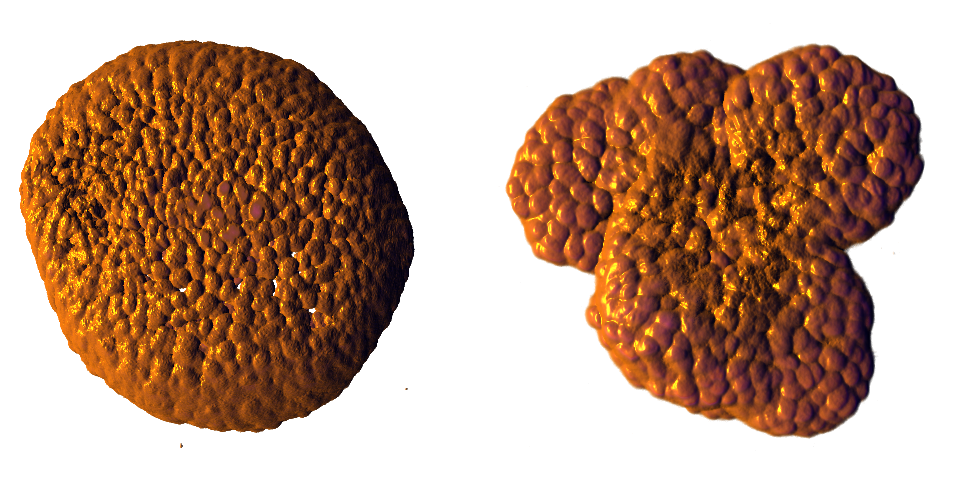
\includegraphics[width=0.85\textwidth]{../img/3Dviz.png}
    \caption{Vision 3D de deux organoïdes représentatifs de notre dataset : organoïde cystique (à gauche) présentant une morphologie saine avec formation d'une cavité centrale, et organoïde choux-fleurs (à droite) caractérisé par une structure plus irrégulière.}
    \label{fig:3Dviz}
\end{figure}

\textbf{Protocole} : Imagerie confocale 8-bit, magnifications 20× et 40×, analyse au 7ème jour de culture (J7)

\textbf{Pipeline} : Images brutes → Segmentation → Nuage de points 3D → Clustering DBSCAN → Création du graphe → Classification GNN

\textbf{Métadonnées} : Chaque organoïde est associé à des coordonnées 3D cellulaires, volumes, connectivité, phénotype

Cette collection, bien que substantielle pour le domaine, reste limitée comparée aux standards du deep learning classique (ImageNet : 14M images), nécessitant des stratégies d'augmentation de données et de transfer learning depuis des données synthétiques.

\subsection{Limites des méthodes actuelles}

\subsubsection{Analyse manuelle : l'expertise au prix de l'échelle}

L'analyse manuelle par des experts biologistes reste actuellement la référence pour l'évaluation d'organoïdes. Un expert peut, en observant un organoïde au microscope ou via des rendus 3D, identifier des caractéristiques phénotypiques subtiles basées sur :
\begin{itemize}
    \item La morphologie globale (forme, taille, régularité)
    \item L'organisation cellulaire (stratification, polarisation)
    \item La présence de structures spécifiques (lumens, bourgeons, cryptes)
    \item L'expression spatiale de marqueurs
\end{itemize}

Cependant, cette approche souffre de limitations majeures qui limitent son utilisation à grande échelle :

\textbf{Limitations pratiques :}
\begin{itemize}
    \item \textbf{Temps d'analyse} : 15-30 minutes par organoïde, rendant impossible l'analyse de milliers d'échantillons
    \item \textbf{Fatigue cognitive} : La qualité d'annotation décroît avec le temps et le nombre d'échantillons
    \item \textbf{Non-automatisable} : Impossibilité d'intégration dans des workflows à haut débit automatisés
\end{itemize}

\textbf{Limitations méthodologiques :}
\begin{itemize}
    \item \textbf{Subjectivité} : Les critères d'évaluation peuvent varier selon l'expertise et l'expérience de l'annotateur
    \item \textbf{Variabilité inter-observateur} : Des experts différents peuvent aboutir à des classifications divergentes
    \item \textbf{Variabilité intra-observateur} : Un même expert peut classifier différemment le même organoïde à différents moments
    \item \textbf{Biais cognitifs} : Des effets d'ancrage et des biais de confirmation peuvent influencer les jugements
\end{itemize}

Ces limitations rendent l'analyse manuelle inadaptée aux études à haut débit modernes où des milliers voire dizaines de milliers d'organoïdes doivent être analysés de manière systématique et reproductible.

\subsubsection{Réseaux de neurones convolutifs 3D : puissance et limitations}

Les réseaux de neurones convolutifs (CNN) ont révolutionné l'analyse d'images 2D en vision par ordinateur et en imagerie biomédicale~\cite{LeCun2015,Krizhevsky2012}. Leur extension naturelle aux volumes 3D (CNN 3D) semble appropriée pour l'analyse d'organoïdes. Cependant, plusieurs limitations majeures freinent leur adoption :

\textbf{Contraintes computationnelles prohibitives :}
\begin{itemize}
    \item \textbf{Empreinte mémoire} : Un CNN 3D sur une image de 2048×2048×200 voxels requiert des dizaines de gigaoctets de mémoire GPU, nécessitant un downsampling massif qui détruit l'information fine
    \item \textbf{Temps d'entraînement} : Les convolutions 3D sont computationnellement coûteuses ($\mathcal{O}(N^4)$ pour un volume $N^3$)
    \item \textbf{Nombre de paramètres} : Les CNN 3D profonds contiennent des millions de paramètres, nécessitant de grandes quantités de données annotées pour éviter le sur-apprentissage
\end{itemize}

\textbf{Limitations méthodologiques :}
\begin{itemize}
    \item \textbf{Perte d'information structurelle} : Les CNN traitent l'organoïde comme une grille de voxels, sans modéliser explicitement les cellules individuelles et leurs relations
    \item \textbf{Sensibilité aux variations d'acquisition} : Les CNN sont sensibles aux changements de luminosité, contraste, résolution, nécessitant une standardisation stricte des protocoles d'imagerie
    \item \textbf{Invariances limitées} : Bien que les CNN possèdent une invariance par translation via la convolution, ils ne sont pas naturellement invariants aux rotations 3D ni aux changements d'échelle sans augmentation de données extensive
    \item \textbf{Manque d'interprétabilité} : Les représentations apprises sont opaques, rendant difficile l'identification des caractéristiques biologiques pertinentes
\end{itemize}

\subsubsection{Descripteurs manuels et machine learning classique}

Une approche alternative consiste à extraire manuellement des descripteurs quantifiant divers aspects des organoïdes, puis à appliquer des algorithmes de machine learning classique (Random Forest, SVM, etc.).

Les descripteurs typiques incluent :

\textbf{Morphologie globale} : Volume, sphéricité, excentricité, surface, compacité

\textbf{Texture} : Matrices de co-occurrence de Haralick (contraste, corrélation, entropie), Local Binary Patterns 3D, moments de Zernike

\textbf{Intensités} : Statistiques d'intensités (moyenne, médiane, écart-type) par canal fluorescent

\textbf{Distribution spatiale} : Gradients radiaux d'intensité, moments d'ordre supérieur

Bien que cette approche soit moins gourmande en données que le deep learning, elle présente des limitations importantes :

\textbf{Ingénierie manuelle} : Le choix et le design des descripteurs nécessitent une expertise domaine importante et sont spécifiques à chaque type d'organoïde

\textbf{Expressivité limitée} : Les descripteurs manuels ne peuvent capturer toute la richesse et la complexité des patterns biologiques

\textbf{Perte d'information relationnelle} : Les relations spatiales entre cellules, cruciales pour comprendre l'organisation tissulaire, sont mal capturées par des statistiques globales

\textbf{Manque de généralisation} : Les descripteurs optimaux pour un type d'organoïde peuvent être inadaptés à un autre
\end{itemize}

\subsection{Besoin d'approches structurelles adaptées}

Face à ces limitations, il apparaît nécessaire de développer des approches qui exploitent explicitement la structure relationnelle des organoïdes plutôt que de les traiter comme de simples images ou volumes.

\subsubsection{Vision relationnelle des organoïdes}

Les cellules au sein d'un organoïde forment un réseau complexe d'interactions :

\textbf{Interactions spatiales} : Contacts directs, proximité géométrique définissant le voisinage cellulaire

\textbf{Interactions fonctionnelles} : Communication paracrine, signalisation, forces mécaniques

\textbf{Organisation hiérarchique} : Gradients de différenciation, polarisation apico-basale, zonation fonctionnelle

Cette organisation relationnelle, plutôt que les propriétés cellulaires individuelles isolées, détermine largement le comportement collectif de l'organoïde et son phénotype macroscopique. Une analyse pertinente devrait donc modéliser explicitement cette structure de réseau.

\subsubsection{Représentations par graphes : une abstraction naturelle}

Les graphes offrent un formalisme mathématique naturel pour représenter les structures relationnelles. Un organoïde peut être modélisé comme un graphe $G = (V, E)$ où chaque cellule constitue un nœud $v_i \in V$ qui est enrichi de features : position 3D, morphologie, intensités de marqueurs et les arêtes $(v_i, v_j) \in E$ encodent les relations de voisinage spatial.

Cette représentation présente plusieurs avantages majeurs :
\textbf{Compression drastique} : Passage de gigaoctets (image brute) à mégaoctets (graphe)

\textbf{Abstraction pertinente} : Focus sur la structure relationnelle biologiquement significative

\textbf{Invariances naturelles} : Les graphes sont naturellement invariants aux transformations géométriques (rotations, translations) une fois les features appropriées définies

\textbf{Flexibilité} : Les graphes peuvent représenter des organoïdes de tailles très variables sans redimensionnement artificiel

\subsubsection{Graph Neural Networks : deep learning sur structures non-euclidiennes}

Les Graph Neural Networks (GNNs)~\cite{Wu2021,Zhou2020,Battaglia2018} constituent l'outil de deep learning adapté aux données structurées sous forme de graphes. En généralisant les opérations de convolution et de pooling aux graphes, les GNNs peuvent :
\begin{itemize}
    \item Apprendre automatiquement des représentations à partir de données
    \item Capturer des patterns structurels complexes et multi-échelles
    \item Exploiter l'information de voisinage local tout en propageant l'information globalement
    \item Maintenir des propriétés d'invariance et d'équivariance géométriques
\end{itemize}

L'application de GNNs à l'analyse d'organoïdes représente une opportunité méthodologique prometteuse, encore peu explorée dans la littérature, qui forme le cœur de cette thèse.

\section{Contributions de la thèse}

\subsection{Contribution 1 : Pipeline automatisé de bout en bout}

Cette thèse propose un pipeline complet et automatisé pour l'analyse d'organoïdes 3D :

\begin{enumerate}
    \item \textbf{Acquisition et prétraitement} : Protocoles d'imagerie optimisés, normalisation d'intensité, débruitage
    \item \textbf{Segmentation cellulaire} : \textbf{Faster Cellpose} 
    \item \textbf{Extraction de features} : propriétés morphologiques pour chaque cellule
    \item \textbf{Construction de graphes} : Graphes géométriques 3D via K-NN
    \item \textbf{Classification par GNN} : Comparaisons de différentes architectures GNN
\end{enumerate}

\subsection{Contribution 2 : Optimisation de la segmentation pour grand débit}

Face à la lenteur de Cellpose original (30 sec/coupe, soit près d'1h30 par oranoïde), nous avons développé deux approches complémentaires de segmentation rapide.

\subsubsection{Méthode géométrique par ellipses}
Nous avons développé une méthode géométrique de segmentation reposant sur la détection déterministe d'ellipses sur les coupes 2D, suivie par un appariement en 3D à l'aide de processus ponctuels marqués. Cette approche permet de réduire le temps de calcul d'un facteur 10 par rapport à Cellpose, ce qui la rend particulièrement adaptée aux besoins de criblage primaire ultra-rapide.

\subsubsection{Faster Cellpose via Knowledge Distillation}
Pour accélérer significativement la segmentation, nous avons optimisé Cellpose en combinant plusieurs techniques complémentaires. Nous avons d'abord appliqué une distillation de connaissances, permettant de transférer les performances d'un modèle teacher vers un modèle student allégé, doté de moitié moins de paramètres. Ce modèle compact a été ensuite épuré par un "pruning" de 30\% de ses poids, ce qui a réduit la complexité du réseau tout en préservant sa précision. Enfin, nous avons affiné le processus d'inférence grâce à l'ajustement de la taille des batchs, l'utilisation du calcul en "mixed precision" et la diminution du nombre d'itérations. L'ensemble de ces optimisations a permis de diviser par cinq le temps de calcul par rapport à Cellpose standard, passant de 2500 heures à 500 heures pour l'analyse de 1500 organoïdes, et rendant ainsi l'expérimentation à grande échelle réalisable.

\subsection{Contribution 3 : Représentation par graphes géométriques et GNNs}

Une contribution majeure de ce travail réside dans la représentation des organoïdes sous forme de graphes géométriques et l'évaluation d'architectures GNN adaptées à cette représentation.

\subsubsection{Graphes géométriques enrichis}

Nous avons choisi de représenter chaque organoïde par un graphe enrichi, dans lequel chaque nœud correspond à une cellule positionnée par ses coordonnées spatiales tridimensionnelles $(x, y, z)$. À ces informations de localisation s’ajoutent des caractéristiques morphologiques pour chaque cellule, telles que le volume, la sphéricité, les axes principaux ou encore la surface. Les liens entre cellules (arêtes du graphe) sont établis sur la base de leur proximité géométrique, à l’aide de méthodes telles que le K-nearest neighbors ou un seuil de rayon défini. Cette modélisation hybride permet de capturer simultanément la géométrie spatiale et les propriétés biologiques des cellules au sein des organoïdes.

\subsubsection{GNNs équivariants pour données géométriques}

Nous exploitons des architectures de Graph Neural Networks équivariantes qui respectent les symétries naturelles :

\textbf{Invariance par translation} : Déplacer l'organoïde dans l'espace ne change pas la prédiction

\textbf{Invariance par rotation} : Orienter l'organoïde différemment ne change pas la prédiction

\textbf{Invariance par réflexion} : Symétries miroir préservées

Ces propriétés d'invariance, garanties par construction architecturale plutôt qu'apprises via augmentation de données, assurent la robustesse des prédictions et l'efficacité de l'apprentissage.

\subsubsection{Avantages de l'approche}

Cette approche offre plusieurs bénéfices par rapport aux méthodes existantes :

\textbf{Efficacité computationnelle} : Réduction d'un facteur 1000 de l'empreinte mémoire par rapport aux CNN 3D

\textbf{Expressivité} : Capture explicite de la structure relationnelle

\textbf{Interprétabilité} : Possibilité d'identifier les cellules individuelles importantes pour la prédiction

\textbf{Flexibilité} : Applicable à des organoïdes de tailles et formes variables sans modification

\textbf{Robustesse} : Invariance géométrique intrinsèque

\subsection{Contribution 4 : Génération de données synthétiques contrôlées}

Pour pallier le manque crucial de données annotées, nous proposons une approche innovante de génération de données synthétiques basée sur la théorie des processus ponctuels spatiaux.

\subsubsection{Processus ponctuels pour simulation réaliste}

En simulant différents processus stochastiques de distribution spatiale de points~\cite{Illian2008,Diggle2013} sur des géométries sphériques, nous générons des arrangements cellulaires aux propriétés statistiques contrôlées et connues :

\textbf{Processus de Poisson homogène} : Distribution aléatoire complète, référence de hasard

\textbf{Processus de Matérn} : Clustering contrôlé, représentant l'agrégation cellulaire

\subsubsection{Construction d'organoïdes synthétiques}

À partir des distributions de points obtenues, nous procédons à la construction d’organoïdes synthétiques en deux étapes principales. D’abord, les centroïdes des cellules sont générés selon le processus ponctuel sélectionné, ce qui permet de contrôler précisément la structure spatiale de l’assemblage cellulaire. Ensuite, à partir de ces positions, nous réalisons une partition de la sphère en diagrammes de Voronoï, aboutissant à des segmentations cellulaires aux frontières réalistes, proches de celles observées expérimentalement.

\subsubsection{Stratégie de pré-entraînement et transfer learning}

Les organoïdes synthétiques, avec leurs labels fixés et leur génération illimitée, permettent :

\textbf{Pré-entraînement} : Apprentissage de représentations générales de patterns spatiaux sur données synthétiques abondantes

\textbf{Fine-tuning} : Adaptation à des phénotypes biologiques réels avec un nombre limité d'exemples annotés

\textbf{Augmentation} : Enrichissement du dataset d'entraînement pour améliorer la robustesse

\textbf{Exploration} : Génération de scénarios rares ou extrêmes difficiles à obtenir expérimentalement

Cette approche de transfer learning~\cite{Pan2010,Weiss2016} du synthétique au réel constitue une contribution méthodologique originale, permettant d'entraîner des modèles performants malgré la rareté des données réelles annotées.

\subsection{Contribution 5 : Étude comparative statistiques spatiales vs GNN}

Pour évaluer rigoureusement les mérites relatifs des approches GNN vis-à-vis des approches statistiques classiques, nous avons mené une étude comparative contrôlée (publication au GRETSI 2025) :

\textbf{Méthode :}
Comparaison sur données synthétiques sphériques avec vérité terrain connue, avec variation de bruit gaussien et poivre-et-sel.

\textbf{Résultats clés :}
\begin{itemize}
    \item Sur les géométries régulières (sphériques) : les statistiques spatiales (K, F, G de Ripley) surpassent les GNN
    \item Sur les géométries complexes/variables (ellipsoïdes) : les GNN généralisent mieux que les statistiques spatiales
    \item Profondeur optimale des GNN : 5-6 couches (trade-off expressivité/overfitting)
\end{itemize}

Cette étude éclaire les conditions d'applicabilité de chaque approche et suggère des directions hybrides futures.

\subsection{Contribution 6 : État de l'art des GNN géométriques}

Cette thèse propose une synthèse exhaustive et structurée des Graph Neural Networks géométriques, développée au \textbf{Chapitre 3}.

\subsubsection{Couverture théorique}

Nous formalisons rigoureusement les fondements mathématiques des GNN géométriques :

\textbf{Groupes de symétries} : $E(n)$ (euclidien), $SE(3)$ (euclidien spécial), $O(3)$ (orthogonal)

\textbf{Invariance vs équivariance} : Définitions formelles et conditions d'applicabilité

\textbf{Garanties théoriques} : Propriétés d'équivariance par construction

\subsubsection{Panorama des architectures}

La revue couvre les architectures majeures de complexité croissante :

\textbf{EGNN} : Messages invariants avec mise à jour équivariante des coordonnées

\textbf{SchNet, DimeNet} : Utilisation d'angles et de triplets

\textbf{PaiNN, NequIP} : Représentations vectorielles/tensorielles équivariantes

\subsubsection{Contributions méthodologiques}

Cette synthèse apporte une \textbf{taxonomie unifiée} selon trois axes (équivariance, représentation, information géométrique), des \textbf{design patterns récurrents} pour construire des GNN équivariants, un \textbf{guide de sélection} pour choisir l'architecture adaptée à chaque problème géométrique, et un \textbf{positionnement} justifiant le choix d'architecture pour les organoïdes.

\section{Organisation du manuscrit}

Ce manuscrit est organisé en six chapitres principaux complétés par cinq annexes techniques, suivant une progression logique du contexte aux contributions.

\subsection{Chapitre 2 : État de l'art}

Le \textbf{Chapitre 2} présente un état de l'art exhaustif structuré en quatre volets complémentaires. Nous y examinons d'abord la biologie des organoïdes, en détaillant leurs différents types, les mécanismes de formation et leurs applications biomédicales. Nous abordons ensuite les techniques d'imagerie 3D, en présentant les modalités d'acquisition disponibles, les défis techniques rencontrés et les contraintes computationnelles associées. Le chapitre propose également une revue critique des méthodes d'analyse existantes, qu'il s'agisse d'approches manuelles, de méthodes par vision par ordinateur, ou de techniques d'apprentissage automatique. Enfin, nous identifions les lacunes des approches actuelles et positionnons nos propres contributions dans ce paysage scientifique. Ce chapitre établit ainsi le contexte scientifique et justifie la nécessité de notre approche.

\subsection{Chapitre 3 : Fondements théoriques}

Le \textbf{Chapitre 3} établit les fondements mathématiques et algorithmiques des Graph Neural Networks. Nous y présentons d'abord la théorie des graphes, incluant les définitions fondamentales, les représentations matricielles, les graphes géométriques et les métriques topologiques. Nous introduisons ensuite les Graph Neural Networks en détaillant le paradigme du message passing et les architectures standards telles que GCN, GAT, GraphSAGE et GIN. Le chapitre explore également les extensions géométriques de ces réseaux, notamment les GNNs E(3)-équivariants comme EGNN, en distinguant les notions d'invariance et d'équivariance et en présentant leurs applications biologiques.

\subsection{Chapitre 4 : Méthodologie}

Le \textbf{Chapitre 4} décrit en détail la méthodologie proposée dans cette thèse. Nous commençons par présenter l'architecture générale de notre approche, en justifiant nos choix de conception. Le chapitre aborde ensuite les protocoles de prétraitement, incluant les méthodes d'imagerie, les techniques de normalisation et la correction d'artefacts. Nous détaillons nos deux contributions méthodologiques pour la segmentation optimisée, avant d'expliquer la construction de graphes géométriques 3D via l'algorithme K-NN. Le chapitre présente également notre approche de génération synthétique basée sur les processus ponctuels et les diagrammes de Voronoï, ainsi que les méthodes de validation employées. Enfin, nous comparons différentes architectures GNN adaptées à notre problématique. Ce chapitre constitue le cœur technique de la thèse, détaillant nos contributions algorithmiques.

\subsection{Chapitre 5 : Résultats}

Le \textbf{Chapitre 5} présente les résultats expérimentaux obtenus au cours de cette thèse. Nous commençons par une étude comparative entre approches statistiques spatiales et GNN, dont les résultats ont été publiés au GRETSI 2025, démontrant la robustesse au bruit et la capacité de généralisation géométrique des GNN. Nous évaluons ensuite les performances des différentes architectures GNN (GAT, DeepSets, EGNN, GCN) sur les données synthétiques, en réalisant des analyses d'ablation pour identifier les composants essentiels et caractériser les trade-offs entre performance brute et robustesse géométrique. Nous reportons ensuite les performances obtenues sur les données réelles (500 organoïdes bien différenciés sélectionnés) via transfer learning et fine-tuning. Une discussion critique analysant les forces, les limitations et le positionnement de notre approche conclut ce chapitre.

\subsection{Chapitre 6 : Conclusion}

Le \textbf{Chapitre 6} conclut le manuscrit en synthétisant les contributions scientifiques et méthodologiques apportées par ce travail. Nous y discutons les limitations et défis persistants de notre approche, avant de proposer des perspectives à court terme incluant des extensions méthodologiques et des validations cliniques. Le chapitre esquisse également des directions de recherche à long terme, notamment l'analyse spatio-temporelle, le développement de modèles génératifs et l'intégration multi-modale de données hétérogènes. Enfin, nous évaluons l'impact scientifique et sociétal potentiel de nos contributions pour la communauté de la biologie des organoïdes et de la médecine personnalisée.

%\subsection{Annexes}

%Les cinq annexes fournissent des compléments techniques et théoriques indispensables à la compréhension approfondie de notre travail. L'\textbf{Annexe A} présente les fondamentaux du deep learning, incluant l'historique du domaine, les architectures classiques, les techniques d'optimisation et les méthodes de régularisation. L'\textbf{Annexe B} offre des compléments sur les graphes et les GNNs, abordant notamment les hypergraphes, le cadre théorique du Geometric Deep Learning et les résultats d'expressivité. L'\textbf{Annexe C} développe la théorie des processus ponctuels, couvrant les processus de Poisson, Cox et Gibbs, les méthodes d'estimation et leur application sur surfaces courbes. L'\textbf{Annexe D} détaille les aspects d'implémentation, incluant les technologies employées, l'architecture logicielle développée, les optimisations effectuées et les mesures prises pour garantir la reproductibilité. Enfin, l'\textbf{Annexe E} décrit les données et benchmarks utilisés, les protocoles d'annotation développés et les modalités d'accès au code source et aux données pour favoriser la reproductibilité de nos résultats.

